\documentclass{article}

\usepackage[american]{babel}
\usepackage[T1]{fontenc}
\usepackage{xcolor, fullpage, hyperref, listings, enumitem, sectsty}
\usepackage{fullpage}
\usepackage{graphicx}
\graphicspath{ {./Graphics/} }

\sectionfont{\color{blue}}  % sets colour of sections
\subsectionfont{\color{blue}}

\setlength{\parindent}{0em}
\setlength{\parskip}{1em}

\hypersetup{
    colorlinks=true,
    linkcolor=blue,
    filecolor=magenta,      
    urlcolor=cyan,
}

\newcommand{\hlite}[1]{%
  \colorbox{yellow!50}{#1} }
\newcommand{\units}{\,\mathrm}
  
\title{\color{blue}\texttt{problem2tex} \\ \normalsize{version = 0.8.6 (2022-01-13)}}

\author{
David Johns, \\ \texttt{david.johns@icewire.ca}
}
\date{Document Date - 2022-01-13}

\begin{document}

\maketitle
\tableofcontents

\section{The need for problem to tex}


Latex is an excellent way to create educational material such as textbooks, examples, exams, and problem sets.  The purpose of \texttt{problem2tex} creating a .tex file is to allow one to create a numerical example (or problem) .prb file so that parameters can change and have the solution be automatically updated for that choice of parameters.  In addition, \texttt{problem2tex} has an expression solver that is used to quickly write the solution for an example (or problem).  

Example usage:\\
\texttt{problem2tex -export=example.tex -random=false -sigDigits=4 example.prb}

\section{Installation and Setup}

For installation/setup of problem2tex, see \href{https://www.icewire.ca}{https://www.icewire.ca}




\section{Running problem2tex}

\subsection{Command Line Options}

The command line options for \texttt{problem2tex} are the following:
\begin{itemize}
\item \texttt{-help}
\begin{itemize}
\item[] Print out help info
\end{itemize}
\item \texttt{-version}
\begin{itemize}
\item[] Print out version info
\end{itemize}
\item \texttt{-export=\textcolor{blue}{path}/filename.tex} 
\begin{itemize}
\item[] where the output should be placed 
\item[] \textcolor{blue}{path} is the directory path that can include .. or . and subdirectories
\end{itemize}
\item \texttt{-random=\textcolor{blue}{option}}
\begin{itemize}
\item[] where option is one of ... (problem to tex option)
\item[] \textcolor{blue}{true}: Parameters are randomized
\item[] \textcolor{blue}{false}: Parameters are the first values in the sets (default setting)
\item[] \textcolor{blue}{positive integer}: Seed for random number generator
\item[] \textcolor{blue}{min}: All smallest numbers 
\item[] \textcolor{blue}{max}: All largest numbers
\item[] \textcolor{blue}{minMax}: Random mix of largest and smallest numbers

\end{itemize}
\item \texttt{-sigDigits=\textcolor{blue}{value}}
\begin{itemize}
\item[] where value is an integer that sets the default number of significant digits in the output (If not specified, then it is set to 4).  RunConfig can also be used to set number of significant digits.
\end{itemize}
\end{itemize}

\subsection{Error Logging}

When running problem2tex, error information is placed as comments at the beginning of the output .tex file.  If things do not work as you expect, check the error log information first as Latex error information can sometimes be misleading.

\subsection{Examples}

problem2tex is a way to make problems have parameters that can change and the solution is re-calculated for that solution.  In addition, the solution is easily written as equations which are then displayed as latex solutions.  For this to work, problem2tex has a built-in expression solver similar to Julia or Matlab.   

This example is available at \href{https://www.icewire.ca/examples/testBasic.zip}{testBasic.zip}

In this example, basic01.prb is a user generated problem file and contains the following text:
\begin{lstlisting}
PARAM{x = [2, 3, 4, 5]}
PARAM{y = [6, 7, 8, 9] }
PARAM{k = [8]}
Given VAL{x,=}, VAL{y,=}, and VAL{k,=} find $z = x^2+y-k$

Solution:
RUN(){z=x^2+y-k}
VAL{z,=}
\end{lstlisting}

For the above problem, $x$, $y$ and $k$ are all parameters where $x$ is any one of 2,3,4 or 5 and
y is any one of 6,7,8 or 9 and k is 8.  For the solution, it is simply written as the equation and a built-in expression solver solves the expression and writes it out in correct Latex form.  The solution in this case is written as 

\begin{lstlisting}
RUN(){z=x^2+y-k}
\end{lstlisting}


and when running with the following command\\
\begin{lstlisting}
problem2tex -export=example.tex example.prb
\end{lstlisting}
a tex file is created that can be included in a latex document.

In the same testBasic.zip file, the second example basic01.prb contains the following text:
\begin{lstlisting}
PARAM{V_1 = [2, 3, 4, 5]# UNITS{V}}
PARAM{R_1 = [6, 7, 8, 9]# UNITS{k \Omega}}
Given VAL{V_1,=} and VAL{R_1,=}, find the current  $I_R = V_1/R_1$

Solution:
RUN(){I_R=V_1/R_1#UNITS{A}}
VAL{I_R,=}
\end{lstlisting}
 
What is interesting here is that units can be assigned to parameters and the expression solver takes into account unit prefixes to generate the correct solution value prefix (i.e, f, p, n, $\mu$, m, k, M, G, etc). 

Also related to units, the units for any variable can be set using the UNITS\{\} command.  In addition, a parameter in CONFIG called defaultUnits can be used to set the default units depending on the first letter of the variable. (see CONFIG settings)

\textbf{NOTE: micro uses \textbackslash mu (and not the letter u)}

A latex file can be used to run problem2tex and then include the resulting .tex files into the document as shown in the example below for the file named basic.tex

\begin{lstlisting}
\documentclass{article}
\usepackage{import}
\newlength{\currentparindent} % used to store current parindent
\newlength{\currentparskip}
\newcommand{\incProb}[1]{
    \immediate\write18{problem2tex -export=Problems/tmp/#1.tex 
    -random=false -sigDigits=4 Problems/#1.prb}
    \setlength{\currentparindent}{\parindent} % store current parindent
    \setlength{\currentparskip}{\parskip}
    \setlength{\parindent}{0em}
    \setlength{\parskip}{0em}
    \import{Problems/tmp/}{#1.tex}
    \setlength{\parindent}{\currentparindent} % restore parindent
    \setlength{\parskip}{\currentparskip}
}
    
\newcommand{\units}{\,\mathrm}
\newcommand{\skipLine}{\vspace{2ex}}

\begin{document}

Question 1:

\incProb{basic01}

\vspace{3ex}

Question 2:

\incProb{basic02}

\end{document}
\end{lstlisting}

For the above example, a new command "\textbackslash incProb" has been defined that is used to bring in problems basic01 and basic02 (both should be in the directory Problems below the main directory with basic.tex).  The command "\textbackslash incProb" first runs problem2tex using the \textbackslash immediate\textbackslash write18 command, next the current paragraph settings are stored, then the paragraph settings are set to no indent and no spacing, then the import of the newly generated .tex file is done and finally, the original paragraph settings are restored.

When the above basic.tex is compiled as a text document, the following output is generated:

\fbox{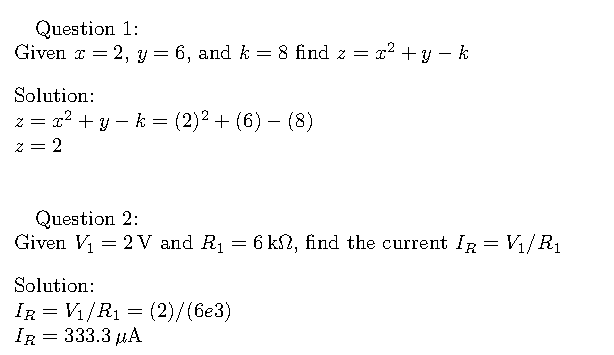
\includegraphics[width=0.6\textwidth]{basicStandAlone}}

In this case, all default parameters are used but it is one line change to obtain random parameters and change the significant number of digits. An example might be ...

\begin{lstlisting}
problem2tex -export=Problems/tmp/#1.tex -random=true -sigDigits=6 Problems/#1.prb
\end{lstlisting}

\subsection{Syntax difference with Latex}

In the above examples, there are 3 main changes from regular latex.  First, the problem2tex commands do not make use of \textbackslash but instead are determined by keywords that are capitalized.  Second, PARAM, CONFIG and RUNSILENT statements are not printed. Finally, the paragraph and line spacing is modified from regular latex (so that non-latex users could easily generate problems as well).  

Each carriage return in the .prb file results in a new paragraph. However, the spacing between paragraphs is the same as regular line spacing.  In addition, if extra blank lines are included in the .prb file, they result in extra spacing in the final output.  So visually, a new paragraph in the final output can be achieved using a blank line.  Note that more blank lines in a row will result in more spacing.


\subsection{Configuration settings}
Configuration settings can be changed at any time and then they are used going forward until
changed again.  Configuration settings can be changed using the CONFIG command.
Each CONFIG command should be on a separate line with no other commands on the same line.

Example: CONFIG\{random = min\}

\begin{itemize}
\item random - choice of false, true, min, max, minMax and positive integer
\begin{itemize}
\item[] - false:  defaults elements chosen
\item[] - true: random elements chosen
\item[] - min: min sized elements chosen 
\item[] - max: max sized elements chosen
\item[] - minMax: random choice of min and max sized elements chosen
\item[] - positive integer: seed for random generator so same elements can be chosen
\end{itemize}
\item fmtVal - format of output values for \textbackslash val
\begin{itemize}
\item[] - set as CONFIG\{format=X\} where X is one of ...\\
(the number of significant digits can be from 1-9)
\begin{itemize}
\item[] - E4 for engineering format with 4 significant digits
\item[] - S4 for scientific format with 4 significant digits
\item[] - D4 for decimal format with 4 significant digits
\item[] - \$ for dollar format (always has 2 digits after decimal point)
\item[] - U4 for SI format (including units) with 4 significant digits
\item[] - DEFAULT IS U4
\end{itemize}
\end{itemize}
\item fmtRun= - format of output values after equal in RUN= or RUN()= commands
\begin{itemize}
\item[] - Same as format above 
\item[] - DEFAULT IS U4
\end{itemize}
\item fmtRun() - format of output values in bracketed numbers in RUN() or RUN()= commands
\begin{itemize}
\item[] - Same as format above
\item[] - DEFAULT IS E4 
\end{itemize}
\item KFactor - Used for default set generation if PARAM sets variable to a nominal number.
\begin{itemize}
\item[] - Set KFactor example: CONFIG\{KFactor = 1.5:5\} where 1.5 is the factor and 5 is the number of elements in the set.  
\item[] - Factor must be a number greater than 1.
\item[] - The range of the elements are from nominal/factor to nominal*factor and are geometrically spaced.
\end{itemize}
\item defaultUnits - used to set the default units depending on the first letter of a variable
\begin{itemize}
\item[] - example: CONFIG\{defaultUnits = [[iI:A][vV:V][R:\textbackslash Omega]]\}
\item[] - above example results in variables starting with the letter i or I having default units of "A"
\item[] - variables starting with letter v or V having default units of "V"
\item[] - variables starting with letter R having default units of "\textbackslash Omega"
\item[] - use of UNITS within a run command will override the default unit setting
\end{itemize}
\item verbose - choice of true or false (default false)
\begin{itemize}
\item[] - prints out the elements sets in commented out lines in the .tex file (useful for debugging)\item[] - Also prints out the configuration settings
\end{itemize}
\end{itemize}

\subsection{Commands for .prb files}

There are 4 main commands for problem to tex:
\begin{itemize}
\item CONFIG (discussed above)
\item PARAM
\item RUN, RUN(), RUN()=
\item VAL
\end{itemize}

\subsubsection{PARAM command}
The command PARAM can be used for setting the randomly generated variables (i.e. parameters).  
Each PARAM command must be on a separate line with no other commands on the same line.

\begin{itemize}
\item PARAM\{var = [x1, x2, x3, ...]\# UNITS\{\textcolor{blue}{units}\} SYMBOL\{\textcolor{blue}{varLatex}\} \}
\begin{itemize}
\item[] - var will be a random selection from the set of x1, x2, x3, ...
\item[] - if random=false, the default value for var is the first element
\item[] - if UNITS\{\textcolor{blue}{units}\} is present, then the units for that variable will be \textcolor{blue}{units}
\item[] - if SYMBOL\{\textcolor{blue}{varLatex}\} is present, then when printing out, the symbol for var will be replaced with \textcolor{blue}{varLatex}
\end{itemize}
\item PARAM\{var = min;max;stepsize\# UNITS\{\textcolor{blue}{units}\} SYMBOL\{\textcolor{blue}{varLatex}\} \}
\begin{itemize}
\item[] - The set for var will be generated from min;max;stepsize
\item[] - The first element will be min so the default will be the min element
\item[] - Otherwise, it is the same as the array generation above
\end{itemize}
\item PARAM\{var = nominal\# UNITS\{\textcolor{blue}{units}\} SYMBOL\{\textcolor{blue}{varLatex}\} \}
\begin{itemize}
\item[] - The set for var will be generated from nominal and the KFactor configuration parameter
\item[] - KFactor: factor:numElements... factor is a number greater than 1 and numElements is a positive integer (numElements is the number of elements in the set).
\item[] - Elements range from nominal/factor to nominal*factor and are geometrically spaced
\item[] - Example: if nominal is 10 and factor is 1.5, then the range is from 6.667 to 15
\item[] - The default is nominal which would be 10 in the above example
\item[] - Otherwise, it is the same as the array generation above
\end{itemize}
\end{itemize}
\subsubsection{RUN commands}

The commands RUN are used for evaluating expressions and setting new variables.

\textbf{The format for an expression is the same as Matlab or Julia (NOT a latex equation).}

See the Expression Solver section below for more information.

Options are the same as in PARAM.

\textbf{In all cases below, the \textcolor{blue}{expr} is evaluated and the result is assigned to \textcolor{blue}{var}}

\begin{itemize}
\item RUN\{\textcolor{blue}{var} = \textcolor{blue}{expr} \# \textcolor{blue}{options} \}
\begin{itemize}
\item[] - Print out \textcolor{blue}{var} = \textcolor{blue}{expr}.  
\item[] - There can be multiple \textcolor{blue}{var} = \textcolor{blue}{expr} separated by ";" 
\end{itemize}
\item RUNSILENT\{\textcolor{blue}{var} = \textcolor{blue}{expr} \# \textcolor{blue}{options}\}
\begin{itemize}
\item[] - Do not print anything out
\end{itemize}
\item RUN()\{\textcolor{blue}{var} = \textcolor{blue}{expr} \# \textcolor{blue}{options}\}
\begin{itemize}
\item[] - Print out \textcolor{blue}{var} = \textcolor{blue}{expr} AND print out intermediate () \textcolor{blue}{expr} for clarity
\end{itemize}
\item RUN=\{\textcolor{blue}{var} = \textcolor{blue}{expr} \# \textcolor{blue}{options}\}
\begin{itemize}
\item[] - Print out \textcolor{blue}{var} = \textcolor{blue}{expr} AND print out  "= result"
\end{itemize}
\item RUN()=\{\textcolor{blue}{var} = \textcolor{blue}{expr} \# \textcolor{blue}{options}\}
\begin{itemize}
\item[] - Print out \textcolor{blue}{var} = \textcolor{blue}{expr} AND print out intermediate () \textcolor{blue}{expr} AND print out "= result"
\end{itemize}
\end{itemize}

\subsubsection{VAL command}
Below is the VAL command for printing out variable value or an expression value.  
\begin{itemize}
\item VAL\{\textcolor{blue}{expr,format}\}
\begin{itemize}
\item[] - Print out the result of \textcolor{blue}{expr} with format set by \textcolor{blue}{format} (see below for format choices)
\item[] - \textcolor{blue}{,format} is optional.  If not present, then the default setting for format is used which was set by CONFIG\{format = X\}
\item[] - \textcolor{blue}{expr} in a \textbackslash val command should NOT contain a ","
\item[] - \textcolor{blue}{expr} in a \textbackslash run command may contain ","s
\item[] - \textcolor{blue}{expr} can be a single variable or a full expression
\end{itemize}
\item VAL format types
\begin{itemize}
\item[] - E4 for engineering format with 4 significant digits
\item[] - S4 for scientific format with 4 significant digits
\item[] - D4 for decimal format with 4 significant digits
\item[] - \$ for dollar format (always has 2 digits after decimal point)
\item[] - U4 for SI format (including units) with 4 significant digits
\item[] - L for only printing VAL latex symbol (not the value of VAL)
\item[] - = for printing "latex symbol = value"
\item[] - DEFAULT IS U4
\end{itemize}

\end{itemize}

\subsection{Expression Solver}

Problem to tex makes use of a built in expression solver to solve \textcolor{blue}{expr} within RUN\{\textcolor{blue}{expr}\}.  Expressions are made similar to Julia or Matlab.  

Example valid  \textcolor{blue}{expr} are:
\begin{itemize}
\item RUN\{A = sqrt(B)*abs(-4)\}
\item RUN\{R\_4 = parll(R\_1,parll(R\_2,R\_3))\}
\end{itemize}

\subsubsection{Functions}

The functions currently available in problem2tex are:

\begin{itemize}
\item[] abs, asin, asinh, acos, acosh, atan, atanh, ceil, cos, cosh, exp, floor, log, log10, round, sin, sinh, sqrt, tan, tanh
\end{itemize}

the above make use of the math package for golang.

In addition, extra functions are:

\begin{itemize}
\item cosd(x), sind(x), tand(x)
\begin{itemize}
\item[] returns cos(x)/sin(x)/tan(x) but x value is in degrees
\end{itemize}
\item acosd(x), asind(x), atand(x)
\begin{itemize}
\item[] returns acos(x)/asin(x)/atan(x) but returns the value in degrees
\end{itemize}
\item dB(x)
\begin{itemize}
\item[] returns 10*log10(x)
\end{itemize}
\item dbV(x)
\begin{itemize}
\item[] returns 20*log10(x)
\end{itemize}
\item parll(a,b)
\begin{itemize}
\item[] returns the numeric parallel value (returns $(1/a + 1/b)^{-1}$)
\item[] the latex printout of this function is $||$ to make it more readable
\end{itemize}
\end{itemize}

\subsubsection{More on Units}

problem2tex will automatically calculate proper unit prefixes IF SI unit notation is used.  For micro, "\textbackslash mu" must be used instead of "u". In some situations, one might want to use a unit notation that is NOT officially SI correct.  For example, one might want to use $\units{V/\mu m}$ instead of $\units{MV/m}$.  In this case a way to achieve this is shown with the following example...

\begin{lstlisting}
PARAM{VAprime = [5,3,4,6]# UNITS{V/\mu m} SYMBOL{V_A'}}
PARAM{V_A = [6, 7, 8, 9]}
Given VAL{VAprime,=} and VAL{V_A,=}, find $L$ 
BEGIN{SOLUTION}
RUNSILENT{VAprime = 1e6*VAprime}
RUN()={L=V_A/VAprime#UNITS{m}}
END{SOLUTION}
\end{lstlisting}

The use of RUNSILENT corrects the value for VAprime (since $\units{\mu m}$ is in the denominator of a unit) by multiplying the values by 1e6. In this example, "L" would default to units of "H" so it is corrected to meters using \textbackslash UNITS\{m\}.

The output becomes ...

\begin{itemize}
% Created with problem2tex: version = 0.8.2 (2021-02-09)
\item[1.] Given \mbox{$V_A' = \mbox{$5 \units{ V/\mu m}$}$} and \mbox{$V_{A} = \mbox{$6 \units{ V}$}$}, find $L$ \\
\textbf{Solution}\\
\mbox{$L=V_{A}/V_A'  = (6)/(5e6) = \mbox{$1.2 \units{\mu m}$}$}\\
\end{itemize}

\section{Graphics}

LTSPICE\{filename\}\{size\}\{horizMove\}\{vertMove\}

SVGLATEX\{filename\}\{size\}\{horizMove\}\{vertMove\}


\section{License}

\subsection{Files created by problem2tex}

All files created by problem2tex are owned by the creators of the work (that is you) and/or by the original authors of the work in cases you use derivative works.

\subsection{Software License}

Copyright \textcopyright\ 2021 David Johns. 

This license applies to problem2tex the program, it's packages, extensions and source code as published or made available through any third party.

Permission is hereby granted, free of charge, to any person obtaining a copy of this software and associated documentation files (the "Software"), to deal in the Software without restriction, including without limitation the rights to use, copy, modify, merge, publish, distribute, sublicense, and/or sell copies of the Software, and to permit persons to whom the Software is furnished to do so, subject to the following conditions:

The above copyright notice and this permission notice shall be included in all copies or substantial portions of the Software.

THE SOFTWARE IS PROVIDED "AS IS", WITHOUT WARRANTY OF ANY KIND, EXPRESS OR IMPLIED, INCLUDING BUT NOT LIMITED TO THE WARRANTIES OF MERCHANTABILITY, FITNESS FOR A PARTICULAR PURPOSE AND NONINFRINGEMENT. IN NO EVENT SHALL THE AUTHORS OR COPYRIGHT HOLDERS BE LIABLE FOR ANY CLAIM, DAMAGES OR OTHER LIABILITY, WHETHER IN AN ACTION OF CONTRACT, TORT OR OTHERWISE, ARISING FROM, OUT OF OR IN CONNECTION WITH THE SOFTWARE OR THE USE OR OTHER DEALINGS IN THE SOFTWARE.


\end{document}
